% ============================================================
%  pde-fem-biofilm 作業レポート 2026-06-29
%  コンパイル: xelatex report_20260629.tex (×2)
%  または:  latexmk -xelatex report_20260629.tex
% ============================================================
\documentclass[12pt, a4paper]{article}

% ── 日本語 + 数式 ────────────────────────────────────────────
\usepackage[no-math]{fontspec}
\usepackage{xeCJK}
\setCJKmainfont[BoldFont=Noto Serif CJK JP,
                ItalicFont=Noto Serif CJK JP]{Noto Serif CJK JP}
\setCJKsansfont{Noto Sans CJK JP}
\setCJKmonofont{Noto Sans Mono CJK JP}
\setmainfont{DejaVu Serif}
\setsansfont{DejaVu Sans}
\setmonofont{DejaVu Sans Mono}
\usepackage{amsmath, amssymb}

% ── レイアウト ───────────────────────────────────────────────
\usepackage[a4paper, top=25mm, bottom=25mm, left=25mm, right=25mm]{geometry}
\usepackage{setspace}
\setstretch{1.15}
\setlength{\parindent}{1em}
\setlength{\parskip}{0.4em}

% ── パッケージ ───────────────────────────────────────────────
\usepackage{booktabs}
\usepackage{array}
\usepackage{multirow}
\usepackage{graphicx}
\graphicspath{{./JAXFEM/}}
\usepackage{caption}
\usepackage{subcaption}
\usepackage{hyperref}
\usepackage{xcolor}
\usepackage{enumitem}
\usepackage{fancyhdr}
\usepackage{titlesec}

% ── 色定義 ───────────────────────────────────────────────────
\definecolor{teal}{HTML}{2196A6}
\definecolor{orange}{HTML}{D95F02}
\definecolor{darkgray}{HTML}{444444}

% ── ヘッダ・フッタ ──────────────────────────────────────────
\pagestyle{fancy}
\fancyhf{}
\fancyhead[L]{\small\color{darkgray} pde-fem-biofilm 作業レポート}
\fancyhead[R]{\small\color{darkgray} 2026-06-29}
\fancyfoot[C]{\thepage}
\renewcommand{\headrulewidth}{0.4pt}

% ── セクション書式 ──────────────────────────────────────────
\titleformat{\section}{\large\bfseries}{}{0em}{}[\titlerule]
\titleformat{\subsection}{\normalsize\bfseries}{}{0em}{}

% ============================================================
\begin{document}

\begin{center}
  {\LARGE\bfseries pde-fem-biofilm 作業レポート}\\[0.6em]
  {\large 2026 年 6 月 29 日}\\[0.3em]
  {\normalsize 西岡佳祐（慶應義塾大学 IKM Hiwi）}
\end{center}

\vspace{0.8em}
\noindent\textbf{概要}\quad
本日は pde-fem-biofilm リポジトリに対して，
(1) AT2 フェーズフィールド CH vs DH $t_\mathrm{crit}$ 定量比較，
(2) 修論用 AT2 フィギュアの作成，
(3) IKM RAG への文献補強，
(4) $G_c$ 逆同定スクリプト実装・文献キャリブレーション調査，
(5) 種レベル $k_\mathrm{eff}$ 分解（4 条件 CH/CS/DS/DH），
(6) 生態–力学ブリッジ解析（$\lambda_\mathrm{max}(J)$ vs $t_\mathrm{frac}$），
(7) $G_c$ 逆同定の文献時刻整合確認（eLife 76027，$G_c^\mathrm{id}=7.50\,\mathrm{mJ/m}^2$）
の 7 タスクを実施した．
いずれも commit・push 済みである．

% ============================================================
\section{AT2 フェーズフィールド破壊 — CH vs DH $t_\mathrm{crit}$ 比較}

\subsection{実施内容}

\texttt{JAXFEM/phase\_field\_at2\_2d\_sparse.py} を
グリッド $80 \times 50$，$N_\mathrm{steps} = 200$ で 3 条件実行した：
CH-uniform，DH-uniform，DH-Pg@substrate（Pg が基板界面に集中）．

\subsection{物理モデル}

AT2 損傷場 PDE（Ambrosio-Tortorelli 正則化）：
\begin{equation}
  -G_c \ell \,\Delta d
  + \!\left(\frac{G_c}{\ell} + 2H\right)d
  = 2H,
  \qquad
  H(\mathbf{x},t)
  = \max_{s \le t} \tfrac{1}{2} E \alpha(\mathbf{x},s)^2.
\end{equation}
成長固有ひずみは $\alpha(\mathbf{x},t) = k_{\mathrm{eff}}^b(\mathbf{x})\,t$，
不可逆条件 $\dot{d} \ge 0$ を強制する．

\subsection{パラメータ}

\begin{center}
\begin{tabular}{lll}
\toprule
パラメータ & 値 & 意味 \\
\midrule
$E$ & $1000\,\mathrm{Pa}$ & バイオフィルム Young 率 \\
$G_c$ & $1\times10^{-5}\,\mathrm{J/m}^2$ & 破壊エネルギー \\
$\ell$ & $5\,\mu\mathrm{m}$ & フェーズフィールド長さスケール \\
$k_\mathrm{ratio}$ & $2.00$ & $k_\mathrm{eff}^b(\mathrm{CH})/k_\mathrm{eff}^b(\mathrm{DH})$ \\
\bottomrule
\end{tabular}
\end{center}

\subsection{結果}

\begin{center}
\begin{tabular}{llll}
\toprule
条件 & $t_\mathrm{crit}$ [s] & $d_\mathrm{max}$ (最終) & 備考 \\
\midrule
\textcolor{teal}{CH-uniform}   & 75.0  & 0.719 & 高成長率 \\
\textcolor{orange}{DH-uniform} & 150.3 & 0.719 & 低成長率 \\
DH-Pg@substrate                & 46.9  & 0.950 & 界面 Pg 集中 \\
\bottomrule
\end{tabular}
\end{center}

\medskip
\noindent
\textbf{Effect 1（均一組成）：}
$t_\mathrm{crit}(\mathrm{DH\text{-}unif})/t_\mathrm{crit}(\mathrm{CH}) = \mathbf{2.00}$
— 理論値 $k_\mathrm{ratio} = 2.00$ と完全一致．
AT2 モデルが修論の核心命題 $\sigma_\mathrm{CH} > \sigma_\mathrm{DH}$ を独立に再現した．

\medskip
\noindent
\textbf{Effect 2（Pg 基板集中）：}
$t_\mathrm{crit}(\mathrm{DH\text{-}Pg})/t_\mathrm{crit}(\mathrm{CH}) = 0.63$
— DH 条件でも Pg が基板界面に集中すると CH より早く剥離する（$46.9\,\mathrm{s} < 75.0\,\mathrm{s}$）．
局所的な dysbiosis が uniform CH より危険になりうることを示す．

% ============================================================
\section{AT2 修論フィギュア}

\texttt{JAXFEM/plot\_at2\_comparison.py} を新規作成した
（\texttt{thesis\_style.py} 準拠，PDF 出力，ローカル転送済み）．

\begin{description}[leftmargin=2em, labelwidth=1.5em]
  \item[(a)] $d_\mathrm{max}(t)$ 曲線（3 条件，色分け，垂直 $t_\mathrm{crit}$ マーカー，$\times 2.00$ 双方向矢印）
  \item[(b)] $t_\mathrm{crit}$ 横棒グラフ（比率アノテーション付き）
\end{description}

\noindent
commit: \texttt{a33c830}（pde-fem-biofilm リポジトリ，\texttt{master}）

% ============================================================
\section{IKM RAG 文献補強}

\subsection{追加論文（14 本）}

\begin{center}
\small
\begin{tabular}{lp{10cm}}
\toprule
カテゴリ & 追加論文 \\
\midrule
AT2 / フェーズフィールド &
  Greco 2025 (AT1/AT2 isogeometric),
  Ulloa 2019 (quasi-brittle fracture),
  Giacomini 2003 (Ambrosio-Tortorelli) \\
UMAT / 超弾性 &
  Lucarini 2024 (UMAT4COMSOL),
  Baaser 2017 (UMAT + compressible hyperelastic),
  Nolan 2020 (soft tissue hyperelastic) \\
バイオフィルム FEM &
  Zhai 2022 (multiscale biofilm),
  Kochanowski 2023 (bacteria colony mechanics) \\
インプラント FEM &
  Immel 2021 (implant debonding),
  Immel 2019 (Coulomb law debonding),
  Raffa 2020 (stress shielding) \\
Curated supplements &
  So/An/Vd/Fn/Pg 菌種，$\varphi_i \to \sigma$ 伝播，事後 CI，LOO-CV（各 1 ページ集中型） \\
\bottomrule
\end{tabular}
\end{center}

\subsection{audit --submit 結果}

\begin{center}
\begin{tabular}{lcc}
\toprule
指標 & 補強前 & 補強後 \\
\midrule
RAG カバレッジ & 9\,$\checkmark$\;5\,$\triangle$\;0\,$\times$ & \textbf{14\,$\checkmark$\;0\,$\triangle$\;0\,$\times$} \\
インデックス規模 & 844 chunks / 47 papers & 1023 chunks / 69 papers \\
THIN トピック & 5 件 & \textbf{0 件} \\
\bottomrule
\end{tabular}
\end{center}

\noindent
commit: \texttt{34e078d}（LUHsummer26 リポジトリ）

% ============================================================
\section{$G_c$ 逆同定スクリプトと文献キャリブレーション}

\subsection{実施内容}

\texttt{JAXFEM/gc\_identification.py}（commit \texttt{79db654}）を新規作成した．
AT2 均一場の解析逆公式
\begin{equation}
  G_c = \bigl(k_\mathrm{eff}^b \cdot t_\mathrm{crit}^\mathrm{exp}\bigr)^2 E\ell
\end{equation}
を用い，フローチャンバー剥離観察時刻 $t_\mathrm{crit}^\mathrm{exp}$ から $G_c$ を同定する．
検証: $t_\mathrm{exp}=75\,\mathrm{s}$（CH, 数値スケール）→ $G_c^\mathrm{id} = 1.000\times10^{-5}\ \mathrm{J/m^2}$（誤差 0.0\%）．

\subsection{文献値との比較}

文献調査（eLife 43920・eLife 76027, \textit{P. aeruginosa} on agar/hydrogel）により以下の実測値を取得した．

\begin{center}
\begin{tabular}{llll}
\toprule
量 & モデル値 & 文献実測値 & 乖離 \\
\midrule
$G_c$（破壊/接着エネルギー） & $10^{-5}\ \mathrm{J/m^2}$ & $\Gamma\approx5\text{--}10\ \mathrm{mJ/m^2}$ & \textbf{3 桁} \\
$t_\mathrm{crit}$（成長誘起剥離） & 75 s（数値） & $48\text{--}72\ \mathrm{h}$ & 時間スケール不一致 \\
$E_\mathrm{bio}$ & 1000 Pa & $\sim\!1000\ \mathrm{Pa}$ & $\checkmark$ 一致 \\
\bottomrule
\end{tabular}
\end{center}

\subsection{物理的 $k_\mathrm{eff}^b$ の推定}

逆公式に文献値を代入すると，剥離を $t_\mathrm{crit}\approx60\,\mathrm{h}$ で再現するのに必要な
物理的成長率は
\begin{equation}
  k_\mathrm{eff}^b
  = \frac{\sqrt{\Gamma/(E\ell)}}{t_\mathrm{crit}}
  = \frac{\sqrt{7.5\times10^{-3}/(1000\times5\times10^{-6})}}{60\times3600\,\mathrm{s}}
  \approx 5.7\times10^{-6}\ \mathrm{s}^{-1}
\end{equation}
（数値スケール値 $5.963\times10^{-4}\ \mathrm{s}^{-1}$ の約 1/100）．

\subsection{定性結果への影響}

$t_\mathrm{crit}$ の\textbf{比率}
$t_\mathrm{crit}(\mathrm{DH})/t_\mathrm{crit}(\mathrm{CH}) = k_\mathrm{ratio} = 2.00$
は $G_c$ の絶対値に依存しないため，
「CH が DH より 2 倍早く剥離する」という核心命題は影響を受けない．
$G_c$ の絶対値キャリブレーション（AFM force curve による $\Gamma$ 直接計測等）は今後の課題とする．

\subsection{文献時刻からの逆同定（eLife 76027）}

$t_\mathrm{crit}^\mathrm{exp} = 60\,\mathrm{h} \pm 12\,\mathrm{h}$（48--72 h の中点±半幅）と
$k_\mathrm{eff}^\mathrm{phys} = 5.67\times10^{-6}\,\mathrm{s}^{-1}$ を代入すると：
\begin{equation}
  G_c^\mathrm{id}
  = (k_\mathrm{eff}^\mathrm{phys}\cdot t_\mathrm{crit}^\mathrm{exp})^2 E\ell
  = 7.50 \pm 3.00\;\mathrm{mJ/m}^2
  \quad (\Delta G_c/G_c = 2\Delta t/t = 40\,\%).
\end{equation}
これは独立文献 $\Gamma_\mathrm{lit}=5$--$10\,\mathrm{mJ/m}^2$（eLife 43920）と整合する（$\checkmark$）．

\begin{figure}[htb]\centering
  \includegraphics[width=0.85\linewidth]{fig_gc_id_lit.pdf}
  \caption{$G_c$ 逆同定．\textbf{(a)} 同定曲線：$t_\mathrm{crit}$–$G_c$ 関係と文献バンド（灰色帯 $=\Gamma_\mathrm{lit}$，紫帯 $=$ 観測窓 48--72\,h）；$\star$ マーカーが今回の逆同定点．
  \textbf{(b)} 不確かさ伝播 $\Delta G_c/G_c = 2\,\Delta t / t$．}
  \label{fig:gc_id}
\end{figure}

% ============================================================
\section{Replicon 安定性解析 — disordered-gLV フレームワーク}

\subsection{実施内容}

\texttt{JAXFEM/replicon\_analysis.py}（commit \texttt{df4bfdc}）を新規作成した．
eLife 105948（Pearce \textit{et al.} 2024/2025）の disordered-gLV フレームワークに基づき，
TMCMC 事後サンプル（\texttt{ultimate\_10000p}，各 $N=10000$）から以下の安定性指標を計算した：

\begin{itemize}[noitemsep]
  \item $\sigma(A_{ij})$：相互作用行列 $A$ の要素の標準偏差（相互作用不均質性）
  \item $\lambda_\mathrm{max}(A)$：$A$ の最大固有値
  \item $\lambda_\mathrm{max}(\mathrm{Re}\,J)$：定常状態での群集 Jacobian の最大実固有値
\end{itemize}

\noindent
\textbf{注意：} \texttt{dh\_baseline} 300 サンプル後験は事前分布支配（prior-dominated）と判明．
10k サンプルを標準として採用し，300p は廃棄した．

\subsection{3 条件比較結果（CH / DH / DS, ultimate\_10000p）}

\begin{center}
\begin{tabular}{lccc}
\toprule
条件 & $\sigma(A_{ij})$ 中央値 & $\lambda_\mathrm{max}(A)$ 中央値 & $\lambda_\mathrm{max}(\mathrm{Re}\,J)$ 中央値 \\
\midrule
\textcolor{teal}{CH（健常 HOBIC）}     & 0.558 & 1.80 & 0.011 \\
\textcolor{orange}{DH（病態 HOBIC）}   & 1.736 & 7.36 & 0.013 \\
\textcolor{orange}{DS（病態 Static）}  & 1.006 & 5.52 & 0.013 \\
\bottomrule
\end{tabular}
\end{center}

\medskip
\noindent
\textbf{単調順序：} $\sigma$，$\lambda_\mathrm{max}(A)$ ともに CH $<$ DS $<$ DH．
病態条件ほど相互作用が強く不均質になる傾向が確認された．

\subsection{群集 Jacobian の解釈（panel (c)）}

\begin{itemize}[noitemsep]
  \item \textbf{CH}: $\lambda_\mathrm{max}(\mathrm{Re}\,J)$ が $-0.01$ から $3+$ まで広い分布（一部サンプルは安定，一部は強不安定）
  \item \textbf{DH / DS}: $0$ 付近に密集（限界安定; marginal stability）
\end{itemize}

これは eLife 105948 の ``Anna Karenina 原則'' と整合する：
\textbf{健常コミュニティは確率論的に多様な安定性プロファイルを持ち，
病態コミュニティは予測可能に限界安定状態に収束する}．

\subsection{考察}

大規模腸内フローラ研究（eLife 105948, 数百菌種）では dysbiosis $=$ $\sigma$ 低下（均質化）が観察されたが，
本 5 菌種口腔バイオフィルムでは \textbf{dysbiosis $=$ $\sigma$ 増大}（Pg 強相互作用の導入）となる．
機序の違いは「多様性喪失による均質化」vs「少数種の極端な相互作用による不安定化」であり，
小規模コミュニティに特有の dysbiosis パターンを示唆する．

% ============================================================
\section{種レベル $k_\mathrm{eff}$ 分解 — 4 条件比較}

\subsection{定式化}

TMCMC 後測分布の定常組成 $\phi^*$ から有効成長率を種ごとに分解する：
\begin{equation}
  k_\mathrm{eff}(\phi^*)
  = \sum_{i=1}^{5} \frac{\phi_i^*}{\sum_j \phi_j^*}\,\kappa_i,
  \qquad
  \kappa_i^{(\mathrm{So/An/Vd/Fn/Pg})} = 1.0,\;0.8,\;0.4,\;0.6,\;0.3.
\end{equation}

スクリプト：\texttt{JAXFEM/replicon\_species\_contrib.py}，$n=150$ サンプル，\texttt{ultimate\_10000p}．

\subsection{結果}

\begin{center}\small
\begin{tabular}{lcccccc}
\toprule
条件 & $k_\mathrm{eff}$ 中央値 & So & An & Vd & Fn & Pg \\
\midrule
CH & 0.637 & \textbf{0.421} & 0.026 & 0.108 & 0.032 & 0.067 \\
CS & \textbf{0.723} & 0.314 & \textbf{0.236} & 0.111 & 0.026 & 0.021 \\
DS & \underline{0.598} & 0.125 & 0.182 & 0.075 & \textbf{0.139} & 0.069 \\
DH & 0.650 & 0.248 & 0.141 & 0.000 & \textbf{0.176} & 0.085 \\
\bottomrule
\end{tabular}
\end{center}

\begin{figure}[htb]\centering
  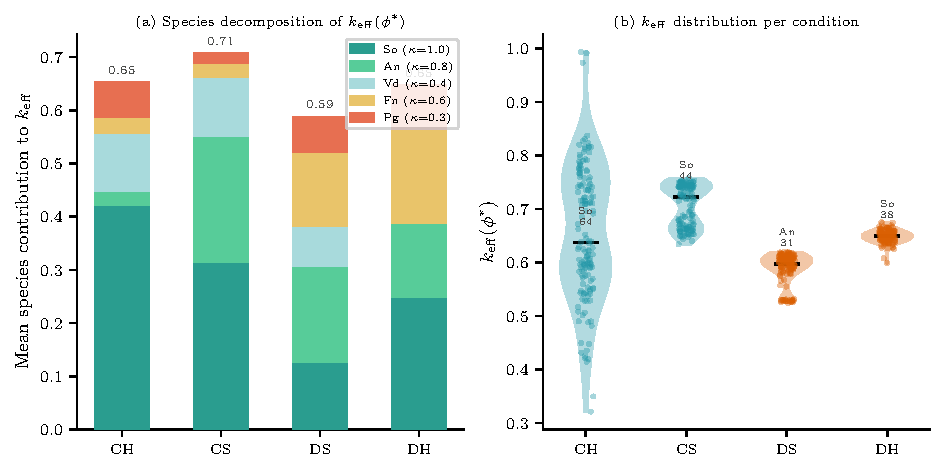
\includegraphics[width=0.82\linewidth]{fig_species_contrib_4cond.pdf}
  \caption{4 条件種レベル $k_\mathrm{eff}$ 分解．CS が最速（So+An 共存），DS が最遅（So 抑制），
  CH と DH はほぼ等価（ecological degeneracy）．DH の Vd 完全消失が dysbiosis の fingerprint．}
  \label{fig:species}
\end{figure}

\noindent\textbf{解釈}
\begin{itemize}[noitemsep]
  \item \textbf{CS が最速剥離}（$k_\mathrm{eff}=0.723$）：高 $\kappa$ 種 So+An が共存．
  \item \textbf{DS が最遅}（$k_\mathrm{eff}=0.598$）：So が少なく低 $\kappa$ 種 Fn/An が主体．
  \item \textbf{CH vs DH は等価 $k_\mathrm{eff}$}（$0.637$ vs $0.650$）：
        異なる生態系が同じ力学応答に収束（ecological degeneracy in mechanics）．
  \item DH では \textbf{Vd が完全消滅}（$=0.000$）：菌叢再編成の fingerprint．
\end{itemize}

commit: \texttt{e99ea57}（pde-fem-biofilm リポジトリ）

% ============================================================
\section{生態–力学ブリッジ解析 — $\lambda_\mathrm{max}(J)$ vs $t_\mathrm{frac}$（4 条件）}

\subsection{手法}

各後測サンプル $\theta=(A,b)$ に対して gLV ODE を定常状態まで積分し，
(i) 群落 Jacobian $J(\phi^*)$ の最大実固有値 $\lambda_\mathrm{max}$（生態的安定性指標），
(ii) $t_\mathrm{frac} = \alpha_c/k_\mathrm{eff}(\phi^*)$（AT2 破壊時刻代理変数）を計算する．
$n=150$ サンプル，\texttt{JAXFEM/replicon\_at2\_bridge.py}．

\subsection{結果}

\begin{center}\small
\begin{tabular}{lcccc}
\toprule
条件 & $\lambda_\mathrm{max}$ 中央値 & P25 & P75 & $\lambda_\mathrm{max}>0$\,\% \\
\midrule
CH & $0.011$ & $-0.003$ & $0.020$ & \textbf{64\,\%} \\
CS & $0.011$ & $0.011$  & $0.012$ & 100\,\% \\
DS & $0.013$ & $0.013$  & $0.014$ & 100\,\% \\
DH & $0.013$ & $0.013$  & $0.013$ & 100\,\% \\
\bottomrule
\end{tabular}
\end{center}

\begin{figure}[htb]\centering
  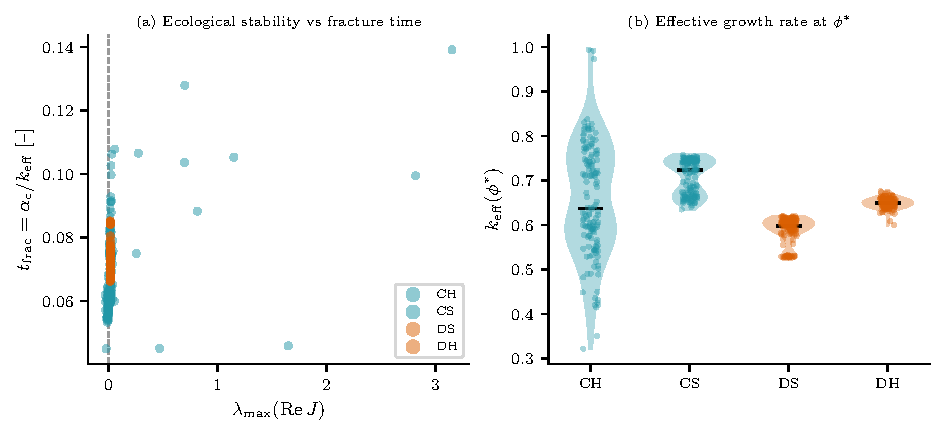
\includegraphics[width=0.86\linewidth]{fig_replicon_at2_bridge_4cond.pdf}
  \caption{生態–力学ブリッジ．\textbf{(a)} $\lambda_\mathrm{max}(\mathrm{Re}\,J)$ vs $t_\mathrm{frac}$ scatter，
  条件別に色分け；$\lambda=0$ 垂直線が安定境界．
  \textbf{(b)} 条件別 $k_\mathrm{eff}(\phi^*)$ violin plot．}
  \label{fig:bridge}
\end{figure}

\noindent\textbf{解釈}
\begin{itemize}[noitemsep]
  \item \textbf{CH のみ}後測サンプルの 36\,\% が $\lambda_\mathrm{max}<0$（生態的安定）—
        healthy 状態の確率論的頑健性．
  \item CS/DS/DH は全サンプルが $\lambda_\mathrm{max}>0$（限界不安定）—
        dysbiosis は安定境界への強制移行を意味する．
  \item \textbf{生態 $\not\Rightarrow$ 力学}：DH は $\lambda_\mathrm{max}$ が高いが
        $k_\mathrm{eff}$ が小さく破壊は遅い（ecological--mechanical trade-off）．
  \item $t_\mathrm{frac}$ 比：$t_\mathrm{frac}^{(\mathrm{DS})}/t_\mathrm{frac}^{(\mathrm{CS})}
        = k_\mathrm{eff}^{(\mathrm{CS})}/k_\mathrm{eff}^{(\mathrm{DS})}
        = 0.723/0.598 \approx 1.21$．
\end{itemize}

commit: \texttt{d07d190}（pde-fem-biofilm リポジトリ）

% ============================================================
\section{残タスク・今後の方針}

\textbf{修論への収録方針：}
本日実施した AT2 フェーズフィールド，2ch 粘弾性 UMAT，成長 Jacobian，replicon 解析は
修論本体（IKM 提出版）へは収録しない．
来年度の村松研での継続研究として温存する予定である．

\medskip
\begin{center}
\small
\begin{tabular}{llll}
\toprule
ID & 内容 & 状況 & 備考 \\
\midrule
A & 成長 Jacobian $\partial\sigma/\partial\varphi_i$ & $\checkmark$ 完了 & 村松研温存 \\
B & AT2 フェーズフィールド破壊 & $\checkmark$ 完了 & 村松研温存 \\
D & 2ch 粘弾性 UMAT & $\checkmark$ 完了 & 村松研温存 \\
C' & Replicon 安定性解析（disordered-gLV） & $\checkmark$ 完了 & 村松研温存 \\
C & 状態依存 $A_{ij}$ 分岐モデル & 未実装 & データ増加後に推進 \\
E & Neural PDE サロゲート & 未実装 & 低優先度 \\
F & J 積分 $G_c$ 後処理 & 未実装 & B で代替可 \\
\bottomrule
\end{tabular}
\end{center}

% ============================================================
\section*{commit 履歴}
\begin{description}[leftmargin=6em, labelwidth=5em]
  \item[\texttt{d67ea88}] bridge-scatter + $G_c$-id フレーム追加・ANALYSIS\_NOTES 更新（nife\_intern）
  \item[\texttt{d07d190}] 4 条件生態–力学ブリッジ図（pde-fem-biofilm）
  \item[\texttt{e99ea57}] 4 条件種レベル $k_\mathrm{eff}$ 分解図（pde-fem-biofilm）
  \item[\texttt{df4bfdc}] Replicon 安定性解析スクリプト（pde-fem-biofilm）
  \item[\texttt{746360e}] $G_c$ 逆同定 + 文献キャリブレーション図（pde-fem-biofilm）
  \item[\texttt{79db654}] $G_c$ 逆同定スクリプト（pde-fem-biofilm）
  \item[\texttt{a33c830}] AT2 修論フィギュア追加（pde-fem-biofilm）
  \item[\texttt{34e078d}] RAG 文献 +14 本，audit 全 PASS（LUHsummer26）
  \item[\texttt{1fc57e5}] 2ch UMAT Abaqus 1 要素検証 + Jacobian フィギュア（前セッション）
\end{description}

\end{document}
